\section{Git Basics}

% \defverbatim[colored]\gitone{
%   \begin{shcode}
%       $ cp -r ex4 myproj
%       $ cd myproj
%       $ git init
%       Initialized empty Git repository in ...
%   \end{shcode}
% }

\defverbatim[colored]\gitone{
  \begin{shcode}
      $ cd myproj
      $ git init
      Initialized empty Git repository in ...
  \end{shcode}
}


\defverbatim[colored]\gitonetwo{
  \begin{shcode}
      $ git config --global user.name "First Last"
      $ git config --global user.email first.last@example.com
      # to list all configuration set for you
      $ git config --list
    \end{shcode}
}

\subsection{Configuration and \texttt{init}}

\begin{frame}
  \frametitle{Configuring \texttt{git} (first time only)}

  To tell git it should log every commit using your name and e-mail, you need
  to configure it once:

  \vspace{2em}

  \gitonetwo

  \begin{exampleblock}{Tip}
    Tab-like auto-completion works out-of-the-box!
  \end{exampleblock}

\end{frame}


\begin{frame}
  \frametitle{Initializing a new repository}

  To initialize a repository just use \texttt{git init}. Let's try it!

  \vspace{2em}

  \gitone

\end{frame}


\defverbatim[colored]\gittwo{
  \begin{shcode}
      $ git status
      On branch master

      Initial commit

      Untracked files:
        (use "git add ...
  \end{shcode}
}

\begin{frame}
  \frametitle{What is staged?}

  The \texttt{status} command gives an overview of the staging area.

  \vspace{2em}

  \gittwo

\end{frame}


\defverbatim[colored]\gitthree{
  \begin{shcode}
      $ git add . #adds all files to staging area
      $ git commit -m "My first commit with git"
      $ git status
      On branch master
      nothing to commit, working directory clean
  \end{shcode}
}

\defverbatim[colored]\gitthreeone{
  \begin{shcode}
      $ git config --global core.editor /usr/bin/nano #default
      $ git config --global core.editor /usr/bin/gedit
      $ git config --global core.editor /usr/bin/vim
      $ git config --global core.editor /usr/bin/gvim
  \end{shcode}
}

\begin{frame}
  \frametitle{Let's do the first commit}

  The \texttt{commit} command instructs git to register the snapshot (patch) to
  its \texttt{.git} directory.

  \vspace{2em}

  \gitthree

  \begin{exampleblock}{Tip: Configuring the default editor}
      \gitthreeone
  \end{exampleblock}

\end{frame}


% \defverbatim[colored]\gitfour{
%   \begin{shcode}
%       $ gedit analysis.py #undo the change
%       # now we use git to problem for the modification
%       $ git diff
%       diff --git a/analysis.py b/analysis.py
%       index d4d5b3e..2697486 100644
%       --- a/analysis.py
%       +++ b/analysis.py
%       @@ -20,4 +20,4 @@ def CER(prediction, true_labels):
%          """

%          errors = (prediction != true_labels).sum()
%       -  return float(errors)/len(prediction)
%       +  return errors/len(prediction)
%   \end{shcode}
% }

\defverbatim[colored]\gitfour{
  \begin{shcode}
      $ #make some changes
      # now we use git to problem for the modification
      $ git diff
      diff --git a/analysis.py b/analysis.py
      index d4d5b3e..2697486 100644
      --- a/analysis.py
      +++ b/analysis.py
      @@ -20,4 +20,4 @@ def CER(prediction, true_labels):
         """

         errors = (prediction != true_labels).sum()
      -  return float(errors)/len(prediction)
      +  return errors/len(prediction)
  \end{shcode}
}

\subsection{Making changes and commits}

\begin{frame}
  \frametitle{Making changes}
  The power of version control can be shown when you make changes.
  % The power of version control can be shown when you make changes. Let's go
  % back to the file \texttt{analysis.py} and undo the fix you just did, so the
  % bug we corrected is re-introduced.

  \vspace{1em}

  \gitfour

  % \textcolor{red}{Note: The commit hashes my differ}

\end{frame}


\defverbatim[colored]\gitfive{
  \begin{shcode}
      $ git commit -m "Re-added nasty bug" -a
  \end{shcode}
}

\begin{frame}
  \frametitle{Committing changes (faster)}

  You can stage and commit changes with one command.

  \vspace{2em}

  \gitfive

\end{frame}


\defverbatim[colored]\gitsix{
  \begin{shcode}
      $ git log --oneline
      df7bc06 Re-added nasty bug
      ccb2d42 My first commit with git
      $ #figured out I re-added the bug, so will revert
      $ git revert df7bc06
      # edit the comment, and save (<ESC>:wq)
      $ git log --oneline
      a43f4c6 Revert "Re-added nasty bug"
      df7bc06 Re-added nasty bug
      ccb2d42 My first commit with git
      $ git diff df7bc06..a43f4c6
      # OK!
  \end{shcode}
}


\begin{frame}
  \frametitle{Recording Changes to the Repository}

  Each file in your working directory can be in one of two states: tracked or untracked.
  Tracked files are files that were in the last snapshot; they can be unmodified, modified, or staged.

  \vspace{1em}

  \begin{center}
    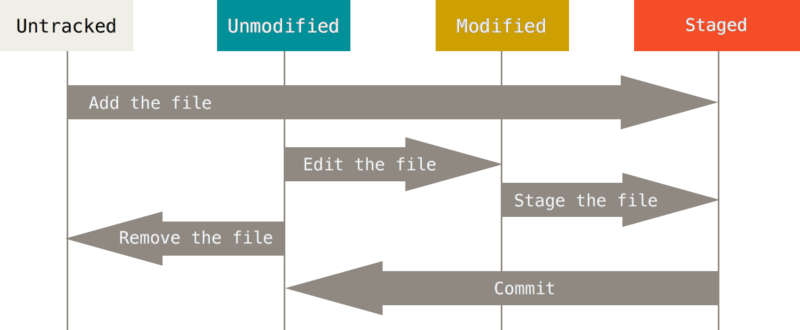
\includegraphics[width=0.9\linewidth]{figures/git-lifecycle}
  \end{center}

\end{frame}

\subsection{Logs, Diffs and Tags}

\begin{frame}
  \frametitle{Logs and Diffs}

  At all times, you have access to history and can revert back.

  \vspace{2em}

  \gitsix

\end{frame}


\defverbatim[colored]\gitseven{
  \begin{shcode}
      $ git tag final #makes final == a43f4c6..
      $ git tag buggy df7bc06 #makes buggy == df7bc06...
      $ git diff buggy..final
      ...
      $ git tag
      buggy
      final
  \end{shcode}
}


\begin{frame}
  \frametitle{Tags}

  Git allows you to set labels to refer to repository versions (instead of
  hash initials). You should use the \texttt{tag} command to do so.

  \vspace{2em}

  \gitseven

\end{frame}

\defverbatim[colored]\gitignore{
  \begin{shcode}
      $ cat .gitignore
      *.[oa]
      *~
  \end{shcode}
}

\subsection{Ignoring Files}
\begin{frame}
  \frametitle{Ignoring Files}

  Git allows you can create a file listing patterns that you want to ignore.
  \vspace{2em}

  \gitignore

  The first line tells Git to ignore any files ending in “.o” or “.a”
  The second line tells Git to ignore all files whose names end with a tilde ($\sim$).
\end{frame}


\begin{frame}
  \frametitle{Rules for \texttt{.gitignore}}

  The rules for the patterns you can put in the .gitignore file are as follows:
  \begin{itemize}
    \item Blank lines or lines starting with \# are ignored.
    \item Standard glob patterns work, and will be applied recursively throughout the entire working tree.
    \item You can start patterns with a forward slash (/) to avoid recursivity.
    \item You can end patterns with a forward slash (/) to specify a directory.
    \item You can negate a pattern by starting it with an exclamation point (!).
  \end{itemize}
\end{frame}

\defverbatim[colored]\gitignoreExample{
  \begin{shcode}
      # ignore all .a files
      *.a
      # but do track lib.a, even though you're ignoring .a files above
      !lib.a
      # only ignore the TODO file in the current directory,
      # not subdir/TODO
      /TODO
      # ignore all files in any directory named build
      build/
      # ignore doc/notes.txt, but not doc/server/arch.txt
      doc/*.txt
      # ignore all .pdf files in the doc/ directory and any of its 
      # subdirectories
      doc/**/*.pdf
  \end{shcode}
}

\begin{frame}
  \frametitle{Ignoring Files}

  Here is another example .gitignore file:

  \vspace{2em}

  \gitignoreExample

\end{frame}

\begin{frame}
  \frametitle{Viewing the Commit History}

  After you have created several commits, or if you have cloned a repository with an existing commit history, you’ll probably want to look back to see what has happened. The most basic and powerful tool to do this is the git log command.
  \vspace{2em}

\end{frame}

